\PassOptionsToPackage{unicode=true}{hyperref} % options for packages loaded elsewhere
\PassOptionsToPackage{hyphens}{url}
\PassOptionsToPackage{dvipsnames,svgnames*,x11names*}{xcolor}
%
\documentclass[10pt,ignorenonframetext,serif,onlymath]{beamer}
\setbeamertemplate{caption}[numbered]
\setbeamertemplate{caption label separator}{: }
\setbeamercolor{caption name}{fg=normal text.fg}
\beamertemplatenavigationsymbolsempty
\usepackage{lmodern}
\usepackage{amssymb,amsmath}
\usepackage{ifxetex,ifluatex}
\usepackage{fixltx2e} % provides \textsubscript
\ifnum 0\ifxetex 1\fi\ifluatex 1\fi=0 % if pdftex
  \usepackage[T1]{fontenc}
  \usepackage[utf8]{inputenc}
  \usepackage{textcomp} % provides euro and other symbols
\else % if luatex or xelatex
  \usepackage{unicode-math}
  \defaultfontfeatures{Ligatures=TeX,Scale=MatchLowercase}
\fi
% use upquote if available, for straight quotes in verbatim environments
\IfFileExists{upquote.sty}{\usepackage{upquote}}{}
% use microtype if available
\IfFileExists{microtype.sty}{%
\usepackage[]{microtype}
\UseMicrotypeSet[protrusion]{basicmath} % disable protrusion for tt fonts
}{}
\IfFileExists{parskip.sty}{%
\usepackage{parskip}
}{% else
\setlength{\parindent}{0pt}
\setlength{\parskip}{6pt plus 2pt minus 1pt}
} 
\usepackage{xcolor}
\usepackage{hyperref}
\hypersetup{
            pdftitle={Euclidean Geometry},
            pdfauthor={Wai-Shing Luk},
            colorlinks=true,
            linkcolor=Maroon,
            citecolor=Blue,
            urlcolor=Blue,
            breaklinks=true}
\urlstyle{same}  % don't use monospace font for urls
\newif\ifbibliography
\usepackage{color}
\usepackage{fancyvrb}
\newcommand{\VerbBar}{|}
\newcommand{\VERB}{\Verb[commandchars=\\\{\}]}
\DefineVerbatimEnvironment{Highlighting}{Verbatim}{commandchars=\\\{\}}
% Add ',fontsize=\small' for more characters per line
\newenvironment{Shaded}{}{}
\newcommand{\AlertTok}[1]{\textcolor[rgb]{1.00,0.00,0.00}{\textbf{#1}}}
\newcommand{\AnnotationTok}[1]{\textcolor[rgb]{0.38,0.63,0.69}{\textbf{\textit{#1}}}}
\newcommand{\AttributeTok}[1]{\textcolor[rgb]{0.49,0.56,0.16}{#1}}
\newcommand{\BaseNTok}[1]{\textcolor[rgb]{0.25,0.63,0.44}{#1}}
\newcommand{\BuiltInTok}[1]{#1}
\newcommand{\CharTok}[1]{\textcolor[rgb]{0.25,0.44,0.63}{#1}}
\newcommand{\CommentTok}[1]{\textcolor[rgb]{0.38,0.63,0.69}{\textit{#1}}}
\newcommand{\CommentVarTok}[1]{\textcolor[rgb]{0.38,0.63,0.69}{\textbf{\textit{#1}}}}
\newcommand{\ConstantTok}[1]{\textcolor[rgb]{0.53,0.00,0.00}{#1}}
\newcommand{\ControlFlowTok}[1]{\textcolor[rgb]{0.00,0.44,0.13}{\textbf{#1}}}
\newcommand{\DataTypeTok}[1]{\textcolor[rgb]{0.56,0.13,0.00}{#1}}
\newcommand{\DecValTok}[1]{\textcolor[rgb]{0.25,0.63,0.44}{#1}}
\newcommand{\DocumentationTok}[1]{\textcolor[rgb]{0.73,0.13,0.13}{\textit{#1}}}
\newcommand{\ErrorTok}[1]{\textcolor[rgb]{1.00,0.00,0.00}{\textbf{#1}}}
\newcommand{\ExtensionTok}[1]{#1}
\newcommand{\FloatTok}[1]{\textcolor[rgb]{0.25,0.63,0.44}{#1}}
\newcommand{\FunctionTok}[1]{\textcolor[rgb]{0.02,0.16,0.49}{#1}}
\newcommand{\ImportTok}[1]{#1}
\newcommand{\InformationTok}[1]{\textcolor[rgb]{0.38,0.63,0.69}{\textbf{\textit{#1}}}}
\newcommand{\KeywordTok}[1]{\textcolor[rgb]{0.00,0.44,0.13}{\textbf{#1}}}
\newcommand{\NormalTok}[1]{#1}
\newcommand{\OperatorTok}[1]{\textcolor[rgb]{0.40,0.40,0.40}{#1}}
\newcommand{\OtherTok}[1]{\textcolor[rgb]{0.00,0.44,0.13}{#1}}
\newcommand{\PreprocessorTok}[1]{\textcolor[rgb]{0.74,0.48,0.00}{#1}}
\newcommand{\RegionMarkerTok}[1]{#1}
\newcommand{\SpecialCharTok}[1]{\textcolor[rgb]{0.25,0.44,0.63}{#1}}
\newcommand{\SpecialStringTok}[1]{\textcolor[rgb]{0.73,0.40,0.53}{#1}}
\newcommand{\StringTok}[1]{\textcolor[rgb]{0.25,0.44,0.63}{#1}}
\newcommand{\VariableTok}[1]{\textcolor[rgb]{0.10,0.09,0.49}{#1}}
\newcommand{\VerbatimStringTok}[1]{\textcolor[rgb]{0.25,0.44,0.63}{#1}}
\newcommand{\WarningTok}[1]{\textcolor[rgb]{0.38,0.63,0.69}{\textbf{\textit{#1}}}}
\usepackage{graphicx,grffile}
\makeatletter
\def\maxwidth{\ifdim\Gin@nat@width>\linewidth\linewidth\else\Gin@nat@width\fi}
\def\maxheight{\ifdim\Gin@nat@height>\textheight\textheight\else\Gin@nat@height\fi}
\makeatother
% Scale images if necessary, so that they will not overflow the page
% margins by default, and it is still possible to overwrite the defaults
% using explicit options in \includegraphics[width, height, ...]{}
\setkeys{Gin}{width=\maxwidth,height=\maxheight,keepaspectratio}
% Prevent slide breaks in the middle of a paragraph:
\widowpenalties 1 10000
\raggedbottom
\setbeamertemplate{part page}{
\centering
\begin{beamercolorbox}[sep=16pt,center]{part title}
  \usebeamerfont{part title}\insertpart\par
\end{beamercolorbox}
}
\setbeamertemplate{section page}{
\centering
\begin{beamercolorbox}[sep=12pt,center]{part title}
  \usebeamerfont{section title}\insertsection\par
\end{beamercolorbox}
}
\setbeamertemplate{subsection page}{
\centering
\begin{beamercolorbox}[sep=8pt,center]{part title}
  \usebeamerfont{subsection title}\insertsubsection\par
\end{beamercolorbox}
}
\AtBeginPart{
  \frame{\partpage}
}
\AtBeginSection{
  \ifbibliography
  \else
    \frame{\sectionpage}
  \fi
}
\AtBeginSubsection{
  \frame{\subsectionpage}
}
\setlength{\emergencystretch}{3em}  % prevent overfull lines
\providecommand{\tightlist}{%
  \setlength{\itemsep}{0pt}\setlength{\parskip}{0pt}}
\setcounter{secnumdepth}{0}

% set default figure placement to htbp
\makeatletter
\def\fps@figure{htbp}
\makeatother

\usetheme{default}
\usepackage{tikz,pgf,pgfplots}
\usetikzlibrary{arrows}
\definecolor{qqqqff}{rgb}{0.,0.,1.}
\newcommand{\columnsbegin}{\begin{columns}}
\newcommand{\columnsend}{\end{columns}}
\newcommand{\col}[1]{\column{#1}}

\title{Euclidean Geometry}
\author{Wai-Shing Luk}
\providecommand{\institute}[1]{}
\institute{Fudan University}
\date{\today}

\begin{document}
\frame{\titlepage}

\begin{frame}
\tableofcontents[hideallsubsections]
\end{frame}
\hypertarget{sec:introduction}{%
\section{Introduction}\label{sec:introduction}}

\begin{frame}{Basic}
\protect\hypertarget{sec:basic}{}

\begin{itemize}
\item
  Line at infinity \(l_\infty = [0, 0, 1]\)
\item
  Two special points \(\mathrm{I}\) and \(\mathrm{J}\) on \(l_\infty\)
  play an important role in Euclidean Geometry:

  \begin{itemize}
  \tightlist
  \item
    \(\mathrm{I} = [1, -i, 0]\), \(\mathrm{J} = [1, i, 0]\)
  \end{itemize}
\item
  \(\mathbf{A} = l_\infty \cdot l_\infty^\mathsf{T}\)
\item
  \(\mathbf{B} = \mathrm{I} \cdot \mathrm{J}^\mathsf{T} + \mathrm{J} \cdot \mathrm{I}^\mathsf{T}\)
\item
  If we choose another line \(l = M \cdot l_\infty\) as line of infinity
\end{itemize}

\end{frame}

\begin{frame}{Notations}
\protect\hypertarget{sec:notations}{}

\begin{itemize}
\tightlist
\item
  To distinguish with Euclidean geometry, points are written in capital
  letters.
\end{itemize}

\end{frame}

\hypertarget{sec:rational-trigonometry-in-euclidean-geometry}{%
\section{Rational Trigonometry in Euclidean
geometry}\label{sec:rational-trigonometry-in-euclidean-geometry}}

\begin{frame}{Quadrance and Spread in Euclidean geometry}
\protect\hypertarget{sec:quadrance-and-spread-in-euclidean-geometry}{}

\begin{itemize}
\item
  The \textbf{quadrance} \(Q\) between points \(A_1\) and \(A_2\) is:
  \[Q = (x'_1 - x'_2)^2 + (y'_1 - y'_2)^2\]
\item
  The \textbf{spread} \(s\) between lines \(l_1\) and \(l_2\) is:
  \[s = (a_1 b_2 - a_2 b_1)^2/(a_1^2 + b_1^2)(a_1^2 + b_1^2)\]
\item
  The \textbf{cross} \(c\) between lines \(l_1\) and \(l_2\) is:
  \[c = 1 - s = (a_1 a_2 + b_1 b_2)^2/(a_1^2 + b_1^2)(a_1^2 + b_1^2)\]
\end{itemize}

\end{frame}

\begin{frame}{Triple formulate}
\protect\hypertarget{sec:triple-formulate}{}

\begin{itemize}
\item
  Let \(A_1\), \(A_2\) and \(A_3\) are points with
  \(Q_1 \equiv Q(A_2, A_3)\), \(Q_2 \equiv Q(A_1, A_3)\) and
  \(Q_3 \equiv Q(A_1, A_2)\). Let \(l_1\), \(l_2\) and \(l_3\) are lines
  with \(s_1 \equiv s(l_2, l_3)\), \(s_2 \equiv s(l_1, l_3)\) and
  \(s_3 \equiv s(l_1, l_2)\).
\item
  Theorem (Triple quad formula): If \(A_1\), \(A_2\) and \(A_3\) are
  collinear points then
  \[(Q_1 + Q_2 + Q_3)^2 = 2(Q_1^2 + Q_2^2 + Q_3^2)\]
\item
  Theorem (Triple spread formula): If \(l_1\), \(l_2\) and \(l_3\) are
  concurrent lines then
  \[(s_1 + s_2 + s_3)^2 = 2(s_1^2 + s_2^2 + s_3^2) + 4 s_1 s_2 s_3.\]
\end{itemize}

\end{frame}

\begin{frame}{Spread Law}
\protect\hypertarget{sec:spread-law}{}

\begin{itemize}
\item
  Suppose that triangle \(\{A_1 A_2 A_3\}\) form quadrances
  \(Q_1 \equiv Q(A_2, A_3)\), \(Q_2 \equiv Q(A_1, A_3)\) and
  \(Q_3 \equiv Q(A_1, A_2)\), and it dual trilateral \(\{l_1 l_2 l_3\}\)
  form spreads \(s_1 \equiv s(l_2, l_3)\), \(s_2 \equiv s(l_1, l_3)\)
  and \(s_3 \equiv s(l_1, l_2)\). Then:
\item
  Theorem (Spread Law) \[\color{Green}{Q_1/s_1 = Q_2/s_2 = Q_3/s_3.}\]
\item
  (Compare with the sine law in Euclidean Geometry):
  \[\color[red}{d_1/\sin \theta_1 = d_2/\sin \theta_2 = d_3/\sin \theta_3}.\]
\end{itemize}

\end{frame}

\begin{frame}{Cross Law}
\protect\hypertarget{sec:cross-law}{}

\begin{itemize}
\item
  Theorem (Cross law)
  \[\color{Green}{(Q_1 + Q_2 - Q_3)^2 = 4 Q_1 Q_2 (1 - s_3)}.\]
\item
  (Compare with the Cosine law)
  \[\color[red}{d_3^2 = d_1^2 + d_2^2 - 2 d_1 d_2 \cos \theta_3}.\]
\end{itemize}

\end{frame}

\begin{frame}{Right triangles and Pythagoras}
\protect\hypertarget{sec:right-triangles-and-pythagoras}{}

\begin{itemize}
\item
  Suppose that \(\{A_1 A_2 A_3\}\) is a right triangle with \(s_3 = 1\).
  Then
\item
  Theorem (Thales) \[s_1 = Q_1 / Q_3 \; \text{and} \; s_2 = Q_2 / Q_3.\]
\item
  Theorem (Pythagoras) \[Q_3 = Q_1 + Q_2.\]
\end{itemize}

\end{frame}

\begin{frame}{Archimedes’ function}
\protect\hypertarget{sec:archimedes-function}{}

\begin{itemize}
\item
  Archimedes’ function \(A(Q_1, Q_2, Q_3)\) \[Ar(Q_1, Q_2, Q_3)
      = (Q_1 + Q_2 + Q_3)^2 - 2(Q_1^2 + Q_2^2 + Q_3^2)\]
\item
  Non-symmetric but more efficient version:
  \[\color{Green}{Ar(Q_1, Q_2, Q_3)
      = 4 Q_1 Q_2 - (Q_1 + Q_2 - Q_3)^2}\]
\end{itemize}

\end{frame}

\begin{frame}{Theorems}
\protect\hypertarget{sec:theorems}{}

\begin{itemize}
\tightlist
\item
  Theorem (Archimedes’ formula): If \(Q_1 = d_1^2\), \(Q_2 = d_2^2\) and
  \(Q_3 = d_3^2\), then \(Ar(Q_1, Q_2, Q_3)\) =
  \[(d_1 + d_2 + d_3) (d_1 + d_2 - d_3) (d_2 + d_3 - d_1) (d_3 + d_1 - d_2)\]
\end{itemize}

\end{frame}

\begin{frame}{Theorems (cont’d)}
\protect\hypertarget{sec:theorems-contd}{}

\begin{itemize}
\item
  Theorem: As a quadratic equation in \(Q_3\), the TQF
  \(Ar(Q_1, Q_2, Q_3) = 0\) can be rewritten as:
  \[Q_3^2 - 2(Q_1 + Q_2) Q_3 + (Q_1 - Q_2)^2 = 0\]
\item
  Theorem: The quadratic equations \[(x - p_1)^2 = q_1\] and
  \[(x - p_2)^2 = q_2\] has a common solutions iff
  \(A(q_1, q_2, (p_1 - p_2)^2) = 0\)
\end{itemize}

\end{frame}

\begin{frame}{Heron’s formula (Hero of Alexandria 60BC)}
\protect\hypertarget{sec:herons-formula-hero-of-alexandria-60bc}{}

\begin{itemize}
\tightlist
\item
  The area of a triangle with side lengths \(a, b, c\) is
  \[\color[red}{\text{area} = \sqrt{s (s - a)(s - b)(s - c)}}\] where
  \(s = (a + b + c)/2\) is the semi-perimeter.
\end{itemize}

\begin{figure}
\hypertarget{fig:heron}{%
\centering
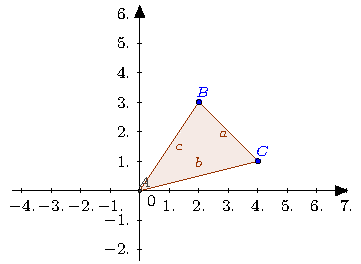
\includegraphics{figs/heron.pdf}
\caption{Heron’s formula}\label{fig:heron}
}
\end{figure}

\end{frame}

\begin{frame}{Archimedes’ theorem}
\protect\hypertarget{sec:archimedes-theorem}{}

\begin{itemize}
\item
  The area of a planar triangle with quadrances \(Q_1, Q_2, Q_3\) is
  given by \[\color{Green}{16(\text{area})^2 = Ar(Q_1, Q_2, Q_3)}\]
\item
  Note: Given \(Q_1, Q_2\). The area is maximum precisely when
  \(Q_3 = Q_1 + Q_2\).
\end{itemize}

\end{frame}

\begin{frame}{Brahmagupta’s formula (convex)}
\protect\hypertarget{sec:brahmaguptas-formula-convex}{}

\begin{itemize}
\item
  Brahmagupta’s theorem:
  \[\color[red}{\text{area} = \sqrt{(s - a) (s - b) (s - c) (s - d)}}\]
  where \(s = (a + b + c + d)/2\)
\item
  Preferred form: \(16\text{area}^2\) =
  \[(-a + b + c + d)(a - b + c + d)
    (a + b - c + d)(a + b + c - d)\]
\end{itemize}

\end{frame}

\begin{frame}{Quadratic compatibility theorem}
\protect\hypertarget{sec:quadratic-compatibility-theorem}{}

\begin{itemize}
\item
  Two quadratic equations
  \[(x - p_1)^2 = q_1, \qquad (x - p_2)^2 = q_2\] are compatible iff
  \[[(p_1 + p_2)^2 - (q_1 + q_2)]^2 = 4 q_1 q_2\] or
  \[Ar(q_1, q_2, (p_1 - p_2)^2) = 0\]
\item
  In this case, if \(p_1 \neq p_2\) then there is a unique sol’n:
  \[2 x = (p_1 + p_2) - (q_1 - q_2)/(p_1 - p_2)\]
\end{itemize}

\end{frame}

\begin{frame}{Quadruple Quad Formula}
\protect\hypertarget{sec:quadruple-quad-formula}{}

\begin{itemize}
\item
  Quadruple Quad Formula \(Q(a,b,c,d)\)
  \[= [(a+b+c+d)^2 - 2(a^2 + b^2 + c^2 + d^2)]^2 - 64 a b c d\]
\item
  Note that \((a+b+c+d)^2 - 2(a^2 + b^2 + c^2 + d^2)\)

  can be computed efficiently as: \[4(ab + cd) - (a + b - c - d)^2\]
\end{itemize}

\end{frame}

\begin{frame}{Brahmagupta’s formula}
\protect\hypertarget{sec:brahmaguptas-formula}{}

\begin{itemize}
\item
  Brahmagupta’s formula (convex): \(B(a,b,c,d)\) =
  \[(b + c + d - a)(a + c + d - b)(a + b + d - c)(a + b + c - d) \]
\item
  Robbin’s formula (non-convex): \(R(a,b,c,d)\) =\\
  \[(a + b + c + d)(a + b - c - d)(a - b + c - d)(b + c - a - d) \]
\item
  Brahmagupta’s identity
  \[Q(a^2,b^2,c^2,d^2) = B(a,b,c,d) \cdot R(a,b,c,d)\]
\end{itemize}

\end{frame}

\begin{frame}{Cyclic quadrilateral quadrea theorem}
\protect\hypertarget{sec:cyclic-quadrilateral-quadrea-theorem}{}

\[(\text{Area})^2 - 2 m (\text{Area}) + p = 0\]

where \[\begin{array}{lll}
    m &=& (Q_{12} + Q_{23} + Q_{34} + Q_{14})^2 - 2(Q_{12}^2 + Q_{23}^2 + Q_{34}^2 + Q_{14}^2)\\
      &=& 4(ab + cd) - (a + b - c - d)^2 \\
      &=& 4(Q_{12}Q_{23} + Q_{34}Q_{14}) - (Q_{12} + Q_{23} - Q_{34} - Q_{14})^2) \\
    p &=& Q(Q_{12}, Q_{23}, Q_{34}, Q_{14})
  \end{array}\]

\end{frame}

\begin{frame}{Ptolemy’s theorem \& generalizations}
\protect\hypertarget{sec:ptolemys-theorem-generalizations}{}

\begin{itemize}
\item
  \textbf{Claudius Ptolemy}: 90-168 A.D. (Alexandria) Astronomer \&
  geographer \& mathematician
\item
  \textbf{Ptolemy’s theorem} If \(\{ABCD\}\) is a cyclic quadrilateral
  with the lengths \(a, b, c, d\) and diagonal lengths \(p, q\), then
  \[a\,b + c\,d = p\,q\] {[}Actually needs convexity!{]}
\end{itemize}

\end{frame}

\begin{frame}{Ptolemy’s theorem}
\protect\hypertarget{sec:ptolemys-theorem}{}

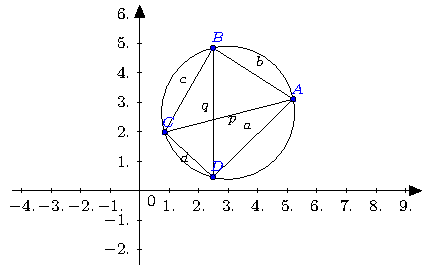
\includegraphics{figs/Ptolemy.pdf}

\end{frame}

\begin{frame}{Exercise}
\protect\hypertarget{sec:exercise}{}

\begin{itemize}
\item
  Ex. \(A_1 = (1,0)\), \(A_2 = (3/5, 4/5)\), \(A_3 = (-12/13, 5/13)\),
  \(A_4 = (15/17, -8/17)\)
\item
  Then the quadrances are:
  \[Q_{12} = 4/5, Q_{23} = 162/65, Q_{34} = 882/221, Q_{14} = 4/17\]
\item
  The diagonal quadrances are: \[Q_{24} = 144/85, Q_{13} = 50/13\]
\end{itemize}

\end{frame}

\begin{frame}{Ptolemy’s theorem (rational version)}
\protect\hypertarget{sec:ptolemys-theorem-rational-version}{}

\begin{itemize}
\item
  Ptolemy’s theorem (rational): If \(\{A_1 A_2 A_3 A_4\}\) is a cyclic
  quadrilateral with quadrances
  \(Q_{ij} \equiv Q(A_i, A_j), i,j=1,2,3,4\) then

  \[\color{Green}{Ar(Q_{12}Q_{34},Q_{23}Q_{14},Q_{13}Q_{24}) = 0}\]
\item
  Ex. For \(A_1 = (1,0)\), \(A_2 = (3/5, 4/5)\),
  \(A_3 = (-12/13, 5/13)\), \(A_4 = (15/17, -8/17)\) with

  \[Q_{12} = 4/5, Q_{23} = 162/65, Q_{34} = 882/221,\]
  \[Q_{14} = 4/17, Q_{24} = 144/85, Q_{13} = 50/13\]
\item
  we can verify directly that
  \(A(Q_{12}Q_{34},Q_{23}Q_{14},Q_{13}Q_{24}) = 0\).
\item
  Note that with the rational form of Ptolemy’s theorem, the three
  quantities appear \emph{symmetrically}: so \emph{convexity} of the
  cyclic quadrilateral is no longer required!
\end{itemize}

\end{frame}

\begin{frame}{Proof of Ptolemy’s theorem}
\protect\hypertarget{sec:proof-of-ptolemys-theorem}{}

Sketch of the proof:

\begin{itemize}
\tightlist
\item
  Without loss of generality, we can assume that the circle is a unit
  circle.
\item
  Recall that a point on a unit circle can be parameterized as:
  \[uc = [\lambda^2 - \mu^2, 2 \lambda \mu, \lambda^2 + \mu^2],\] where
  \(\lambda\) and \(\mu\) are not both zero.
\item
  Let \(A_i = uc(\lambda_i, \mu_i), i = 1, 2, 3, 4\).
\item
  Express \(Q_{ij} \equiv Q(A_i, A_j), i,j=1,2,3,4\) in terms of
  \(\lambda\)’s and \(\mu\)’s
\item
  Express \(Ar(Q_{12}Q_{34},Q_{23}Q_{14},Q_{13}Q_{24})\) in terms of
  \(\lambda\)’s and \(\mu\)’s.
\item
  Simplify the expression and derive that it is equal to 0. (we may use
  the Python’s symbolic package for the calculation. It took about 8
  minutes on my computer :-)
\end{itemize}

\end{frame}

\begin{frame}[fragile]{Python Code}
\protect\hypertarget{sec:python-code}{}

\scriptsize

\begin{Shaded}
\begin{Highlighting}[]
\ImportTok{from}\NormalTok{ __future__ }\ImportTok{import}\NormalTok{ print_function}
\ImportTok{from}\NormalTok{ pprint }\ImportTok{import}\NormalTok{ pprint}
\ImportTok{import}\NormalTok{ numpy }\ImportTok{as}\NormalTok{ np}
\ImportTok{from}\NormalTok{ fractions }\ImportTok{import} \OperatorTok{*}
\ImportTok{from}\NormalTok{ proj_geom }\ImportTok{import} \OperatorTok{*}

\KeywordTok{def}\NormalTok{ quad1(x1, z1, x2, z2):}
    \ControlFlowTok{if} \BuiltInTok{isinstance}\NormalTok{(x1, }\BuiltInTok{int}\NormalTok{):}
        \ControlFlowTok{return}\NormalTok{ (Fraction(x1,z1) }\OperatorTok{-}\NormalTok{ Fraction(x2,z2))}\OperatorTok{**}\DecValTok{2}
    \ControlFlowTok{else}\NormalTok{:}
        \ControlFlowTok{return}\NormalTok{ (x1}\OperatorTok{/}\NormalTok{z1 }\OperatorTok{-}\NormalTok{ x2}\OperatorTok{/}\NormalTok{z2)}\OperatorTok{**}\DecValTok{2}

\KeywordTok{def}\NormalTok{ quadrance(a1, a2):}
    \ControlFlowTok{return}\NormalTok{ quad1(a1[}\DecValTok{0}\NormalTok{], a1[}\DecValTok{2}\NormalTok{], a2[}\DecValTok{0}\NormalTok{], a2[}\DecValTok{2}\NormalTok{]) }\OperatorTok{+} \OperatorTok{\textbackslash{}}
\NormalTok{            quad1(a1[}\DecValTok{1}\NormalTok{], a1[}\DecValTok{2}\NormalTok{], a2[}\DecValTok{1}\NormalTok{], a2[}\DecValTok{2}\NormalTok{])}

\KeywordTok{def}\NormalTok{ uc_point(lambda1, mu1):}
    \ControlFlowTok{return}\NormalTok{ pg_point([lambda1}\OperatorTok{**}\DecValTok{2} \OperatorTok{-}\NormalTok{ mu1}\OperatorTok{**}\DecValTok{2}\NormalTok{,}
                \DecValTok{2}\OperatorTok{*}\NormalTok{lambda1}\OperatorTok{*}\NormalTok{mu1, lambda1}\OperatorTok{**}\DecValTok{2} \OperatorTok{+}\NormalTok{ mu1}\OperatorTok{**}\DecValTok{2}\NormalTok{])}

\KeywordTok{def}\NormalTok{ Ar(a, b, c):}
    \CommentTok{''' Archimedes's function '''}
    \ControlFlowTok{return}\NormalTok{ (}\DecValTok{4}\OperatorTok{*}\NormalTok{a}\OperatorTok{*}\NormalTok{b) }\OperatorTok{-}\NormalTok{ (a }\OperatorTok{+}\NormalTok{ b }\OperatorTok{-}\NormalTok{ c)}\OperatorTok{**}\DecValTok{2}
\end{Highlighting}
\end{Shaded}

\end{frame}

\begin{frame}[fragile]{Python Code (II)}
\protect\hypertarget{sec:python-code-ii}{}

\scriptsize

\begin{Shaded}
\begin{Highlighting}[]
\ControlFlowTok{if} \VariableTok{__name__} \OperatorTok{==} \StringTok{"__main__"}\NormalTok{:}
    \ImportTok{import}\NormalTok{ sympy}
\NormalTok{    sympy.init_printing()}

\NormalTok{    lambda1, mu1 }\OperatorTok{=}\NormalTok{ sympy.symbols(}\StringTok{"lambda1 mu1"}\NormalTok{, integer}\OperatorTok{=}\VariableTok{True}\NormalTok{)}
\NormalTok{    lambda2, mu2 }\OperatorTok{=}\NormalTok{ sympy.symbols(}\StringTok{"lambda2 mu2"}\NormalTok{, integer}\OperatorTok{=}\VariableTok{True}\NormalTok{)}
\NormalTok{    lambda3, mu3 }\OperatorTok{=}\NormalTok{ sympy.symbols(}\StringTok{"lambda3 mu3"}\NormalTok{, integer}\OperatorTok{=}\VariableTok{True}\NormalTok{)}
\NormalTok{    lambda4, mu4 }\OperatorTok{=}\NormalTok{ sympy.symbols(}\StringTok{"lambda4 mu4"}\NormalTok{, integer}\OperatorTok{=}\VariableTok{True}\NormalTok{)}
\NormalTok{    a1 }\OperatorTok{=}\NormalTok{ uc_point(lambda1, mu1)}
\NormalTok{    a2 }\OperatorTok{=}\NormalTok{ uc_point(lambda2, mu2)}
\NormalTok{    a3 }\OperatorTok{=}\NormalTok{ uc_point(lambda3, mu3)}
\NormalTok{    a4 }\OperatorTok{=}\NormalTok{ uc_point(lambda4, mu4)}
\NormalTok{    q12 }\OperatorTok{=}\NormalTok{ quadrance(a1, a2)}
\NormalTok{    q23 }\OperatorTok{=}\NormalTok{ quadrance(a2, a3)}
\NormalTok{    q34 }\OperatorTok{=}\NormalTok{ quadrance(a3, a4)}
\NormalTok{    q14 }\OperatorTok{=}\NormalTok{ quadrance(a1, a4)}
\NormalTok{    q24 }\OperatorTok{=}\NormalTok{ quadrance(a2, a4)}
\NormalTok{    q13 }\OperatorTok{=}\NormalTok{ quadrance(a1, a3)}
\NormalTok{    t }\OperatorTok{=}\NormalTok{ Ar(q12}\OperatorTok{*}\NormalTok{q34, q23}\OperatorTok{*}\NormalTok{q14, q13}\OperatorTok{*}\NormalTok{q24)}
\NormalTok{    t }\OperatorTok{=}\NormalTok{ sympy.simplify(t)}
    \BuiltInTok{print}\NormalTok{(t) }\CommentTok{# get 0}
\end{Highlighting}
\end{Shaded}

\end{frame}

\begin{frame}[fragile]{Backup}
\protect\hypertarget{sec:backup}{}

\begin{verbatim}
>  pandoc -t latex -F pandoc-crossref -o temp2.svg .\01proj_geom.md .\02ck_geom.md .\03RT.md .\04RT_2.md latex.yaml .\crossref.yaml
>  pandoc -t beamer -F pandoc-crossref -o temp2.svg .\01proj_geom.md .\02ck_geom.md .\03RT.md .\04RT_2.md beamer.yaml .\crossref_2.yaml
\end{verbatim}

\end{frame}

\hypertarget{sec:questions}{%
\section{Questions?}\label{sec:questions}}

\end{document}
